\begin{figure}[htbp]
\centering
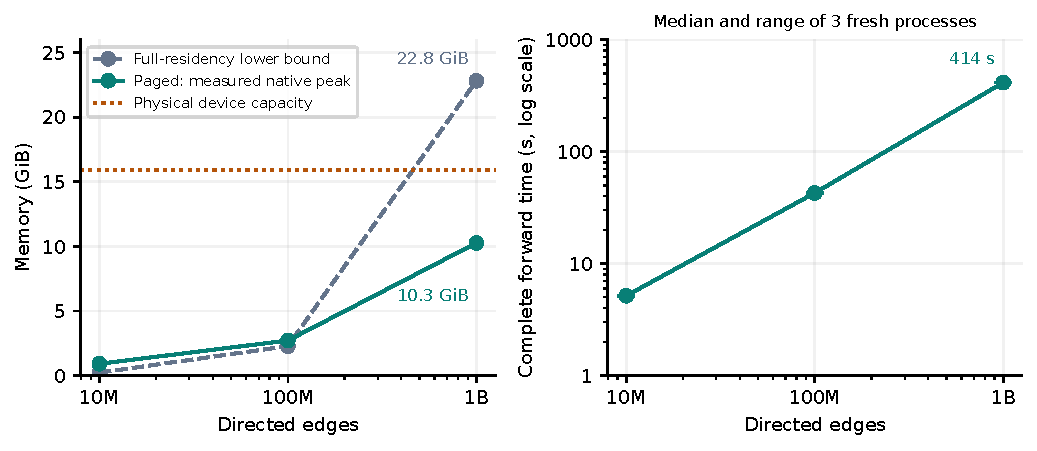
\includegraphics[width=\linewidth]{figures/billion-capacity.pdf}
\caption{One billion explicit edges on a single RTX 5070 Ti. Left: measured
native allocation peak versus the calculated full-residency lower bound, not
an executed resident baseline. Right: median and range of three complete
forward calls in fresh processes, including host staging and output assembly.}
\label{fig:billion}
\end{figure}
All nine trials complete with zero elementwise error. At one billion edges, the median forward takes 414.25 s (range 411.36--415.61 s). The maximum native GPU allocation peak across trials is 10.27 GiB, including the 7.45 GiB output; forward process peak RSS is 8.83 GiB. The maximum sampled whole-device usage is 13.25 GiB, including existing services and runtime pools; one-second sampling is not an exact physical peak. Each trial checks all two billion FP32 output values outside the forward timing interval.
